\documentclass{standalone}

\begin{document}

\chapter[Big Data]{Biological Big Data - CHIMeRA project}\label{chapter3:bigdata}

\begin{center}
\begin{figure}[htbp]
\centering
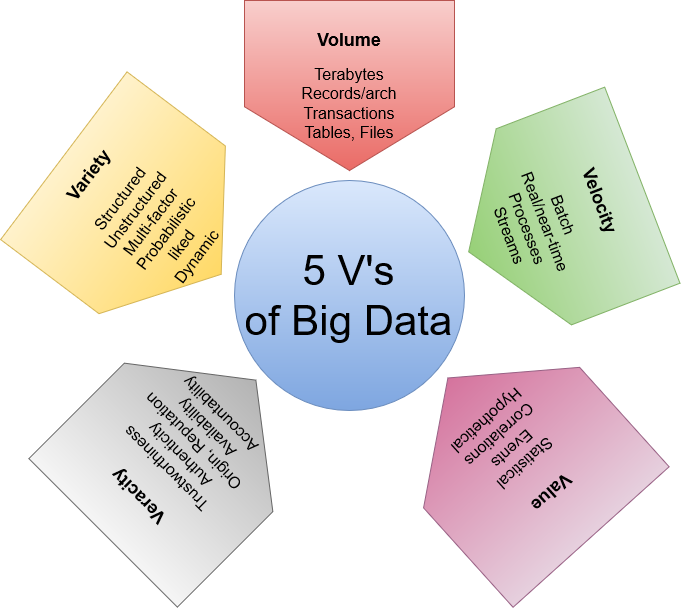
\includegraphics[width=\textwidth]{5v.png}
\caption{Big Data 5 V's}
\label{fig:5v}
\end{figure}
\end{center}

Every second a large quantity of data are produced and shared through Internet and Web-pages.
Data are collected by social networks, messages, video streaming and images.
Everyone, in fact, can easily create new data sources and share or put them in Internet pages.
The growth of this data is not limited to multimedia data but it involves many different fields.
This is one of the most important feature of the contemporary time, the so-called Big Data era: this huge volume of data has created a new field in data processing which is called Big Data Analytics that nowadays positioned among top ten strategic technologies (Gartner Research, 2012).

It is still difficult to provide a definition of what exactly are the Big Data and we can find many slight different nomenclatures and categories which aim to formulate it.
Moreover, Big Data does not define a particular data type but more than we normally think sources can be labeled as it.
The \emph{International Journal of Computer Applications} defined them as \quotes{$[\cdots]$ a collection of large and complex datasets that cannot be processed and analyzed using traditional computing techniques. It is not a single technique or a tool, rather it involves many areas of business and technology}.
This definition certainly involves many aspects of Big Data processing but it does not provide any definition about their nature.
Moreover, it is easy to identify them as \quotes{big} and thus difficult to analyze, but they are all around us every day and just using the Internet connection every smart-phone or laptop can extract and visualize our web queries so could be not properly correct to define them in this way.
However it is certainly sure that the standard computing techniques have to be reviewed to face on this vast amount of data and a even more important attention has to be payed on the algorithm implementations.

While a global definition of them is evidently difficult we can however describe them using some of their \quotes{essential} features.
One of the most common and used set of labels is given by the so called 5 V's of Big Data: volume, velocity, variety, veracity and value.
Despite the first twos are quite obvious (the Big Data are certainly \emph{big} in volume and they are produced very \emph{fast}), the remaining three need a particular attention.
Moreover, we have already treated problems about the volume of data (ref. Chapter\ref{chapter1:featsel}) and the need of very fast processing and algorithm optimizations (ref. Chapter\ref{chapter2:neural}).
Now in this chapter we want to focus on the remaining three characteristics of Big Data Analytics.

As pre-announced there many different sources able to provide data and this feature describes the extreme heterogeneity and variety of them.
We can however broadly classify this variety into three global classes: \emph{structured data}, \emph{semi-structured data} and \emph{unstructured}.
A dataset is \emph{structured} if we can easily manage the informations in it or, in other words, if it is described using the standard formats of data and thus can it can be \quotes{quearable}.
On the other side we have the completely \emph{unstructured} dataset in which the data are disorganized and we need one or multiple pre-processing steps before use them or we have to develop different techniques to handle them.
The intermediate step is given by the \emph{semi-structured} data in which only a part of them could be handle with standard techniques or can be easily brought to their structured version.
The data organization has been a crucial task on this work of thesis and we will return on this topic in the next sections.

The fourth essential characteristic of Big Data is the \emph{veracity} of them due to data inconsistency and incompleteness.
The data are shared very fast using Internet and there could be found some ambiguities and/or deceptions between different data sources.
If we want to merge and aggregate different kind of informations we have also to face on this kind of problems.
The final task of every Big Data Analytic application is, in fact, to process these large quantities of data and obtain a unique answer which can not vary in relation to the portion of data or dataset used.

The last and probably most important feature is certainly their \emph{value}: it is certainly good to have access to large amount of data but unless we can turn them into value they are useless.
In this vast amount of data only a small part of them can be considered as informative and it is always harder to extract this core of informations from them.
Moreover, we have to take into account also the difficulties about the management of these data and their more or less complex structure.
However, also in this case, it is hard to generalize this property on all the amount of data contained in Internet: every day we see a large quantity of useless information on the web and it is hard to figure out that some of them can be useful for research applications.
A key role is played by the \emph{questions} which we ask: for every data source there is always an appropriated question which can be answer using it and vice versa.
In this way also the seemingly useless datasets can acquire importance for an appropriated research project.

In this chapter we will discuss about one of the latest project developed during my PhD and which is still in work in progress: the CHIMera (\emph{Complex Human Interactions in MEdical Records and Atlases}) project.
The project is founded on Big Data applications and it is accidentally born as separated branch of the INFN FiloBlu project (ref. next sections and Appendix E for further informations about the project) which financed my last PhD year.
CHIMeRA aims to create a unified database of bio-medical records using Natural Language processing techniques.
The final purpose is to merge multiple data sources available on-line into a single network structure which highlights the relevant interactions between bio-medical informations, i.e starting from diseases to the biological agents involved into their causes and consequences.
The realization of the first version of CHIMeRA required a lot of time and the development of novel pipelines of data processing.
The project does not still achieve its conclusions but in this chapter we will cross through the main key points which allowed its construction.

%talk about data structured and unstructured
%Many public datasets available.
%Description of the database used in chimera.
%Problems about the intersections and partial informations (single db).


\end{document}
